\documentclass[aspectratio=169]{beamer}
\usepackage{fontawesome5}
\usetheme{metropolis}  
%\usecolortheme{owl}         % Use metropolis theme
\title{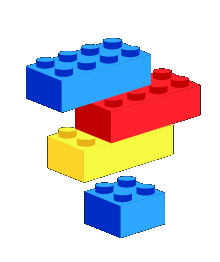
\includegraphics[width=1cm]{img/scafiblocks-logo.png} ScaFi-Blocks}

\subtitle{A Visual Aggregate Programming Environment for Low-Code Swarm Design}
\date{\today}
\author{\alert{Gianluca Aguzzi}, Roberto Casadei, Mirko Viroli}
\institute{University of Bologna, Cesena \\ Talk @ \alert{COORDINATION 2024}}
\newcommand{\hsplit}[2]{
\begin{minipage}{0.48\textwidth}
#1
\end{minipage}
\hfill
\begin{minipage}{0.48\textwidth}
#2
\end{minipage}
}
\newcommand{\hsplits}[4]{
\begin{minipage}{#1\textwidth}
#3
\end{minipage}
\hfill
\begin{minipage}{#2\textwidth}
#4
\end{minipage}
}


\newcommand{\lbl}[1]{\textbf{\textcolor{gray!90!white}{#1}}}
\newcommand{\bo}[1]{\textbf{#1}}

\begin{document}
  \maketitle

  \begin{frame}[fragile]{Swarm Behaviours}

	\begin{alertblock}{Definition}
		\begin{itemize}
			\item 
			\textbf{Swarm behaviours} emerge from the interactions among \underline{a large number} of simple agents.
		
		\end{itemize}
	\end{alertblock}
	\begin{exampleblock}{Examples}
		\begin{itemize}
			\item Collective pattern formation: e.g., flocking, schooling, herding.
			\item Task allocation: e.g., foraging, patrolling, cleaning.
			\item Information dissemination: e.g., gossiping, routing, aggregation.
		\end{itemize}

	\end{exampleblock}
	\begin{center}
	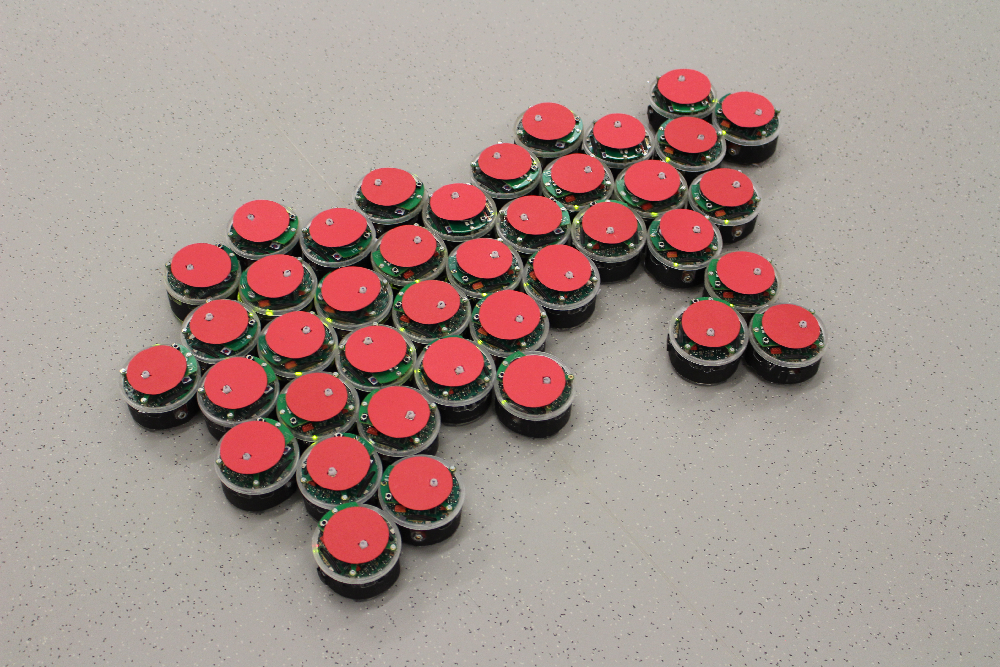
\includegraphics[height=1.6cm]{img/aggregation.jpg}
	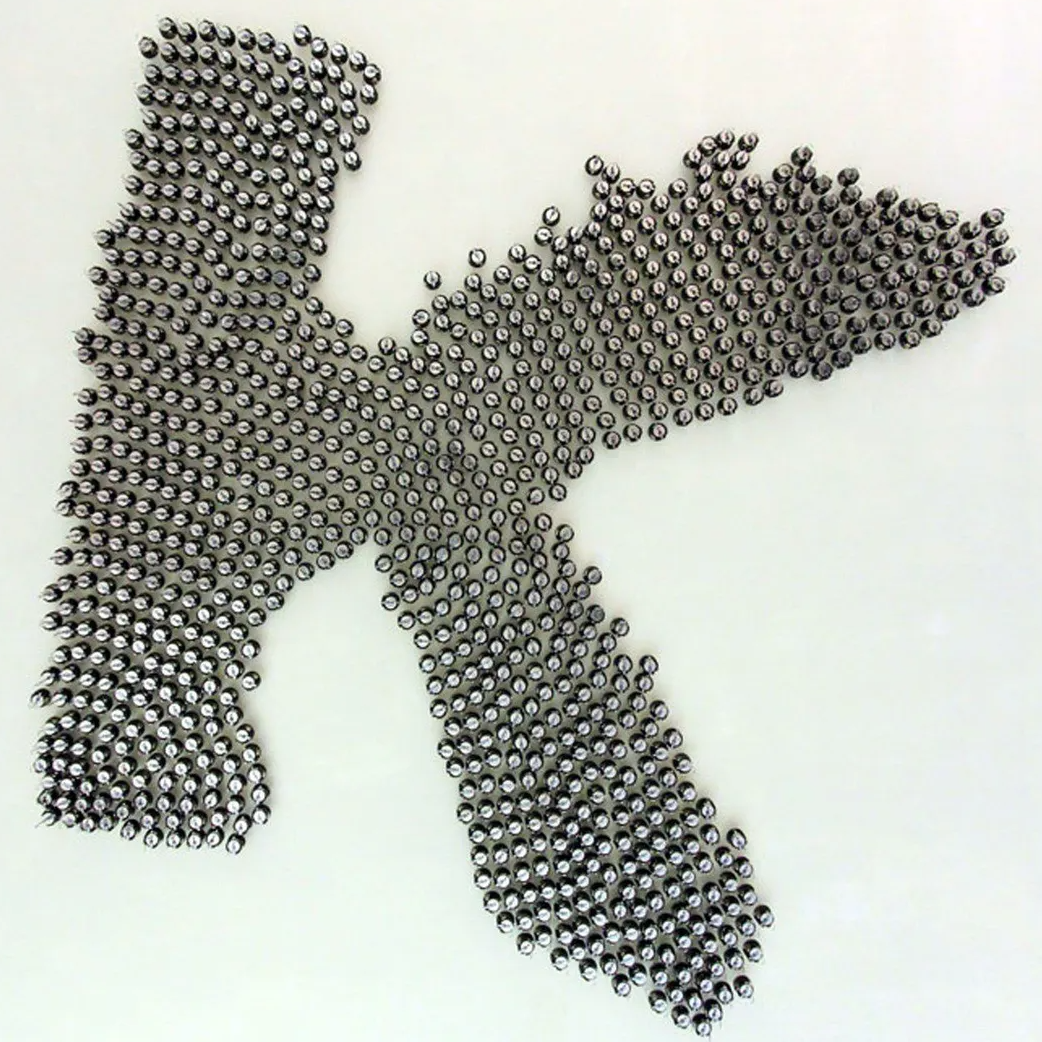
\includegraphics[height=1.6cm]{img/pattern-formation.png}
	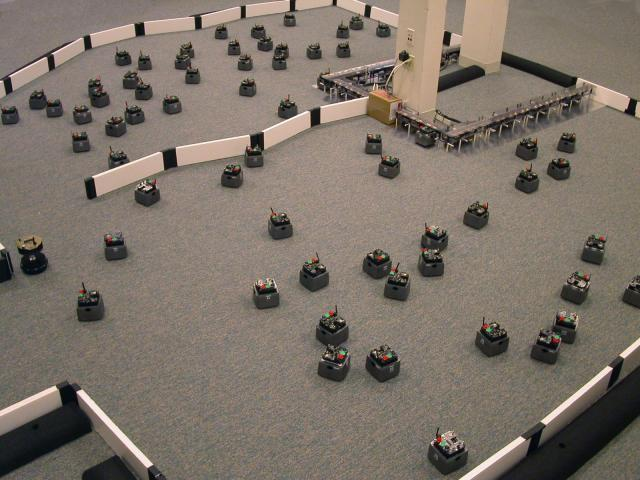
\includegraphics[height=1.6cm]{img/exploration.jpg}
	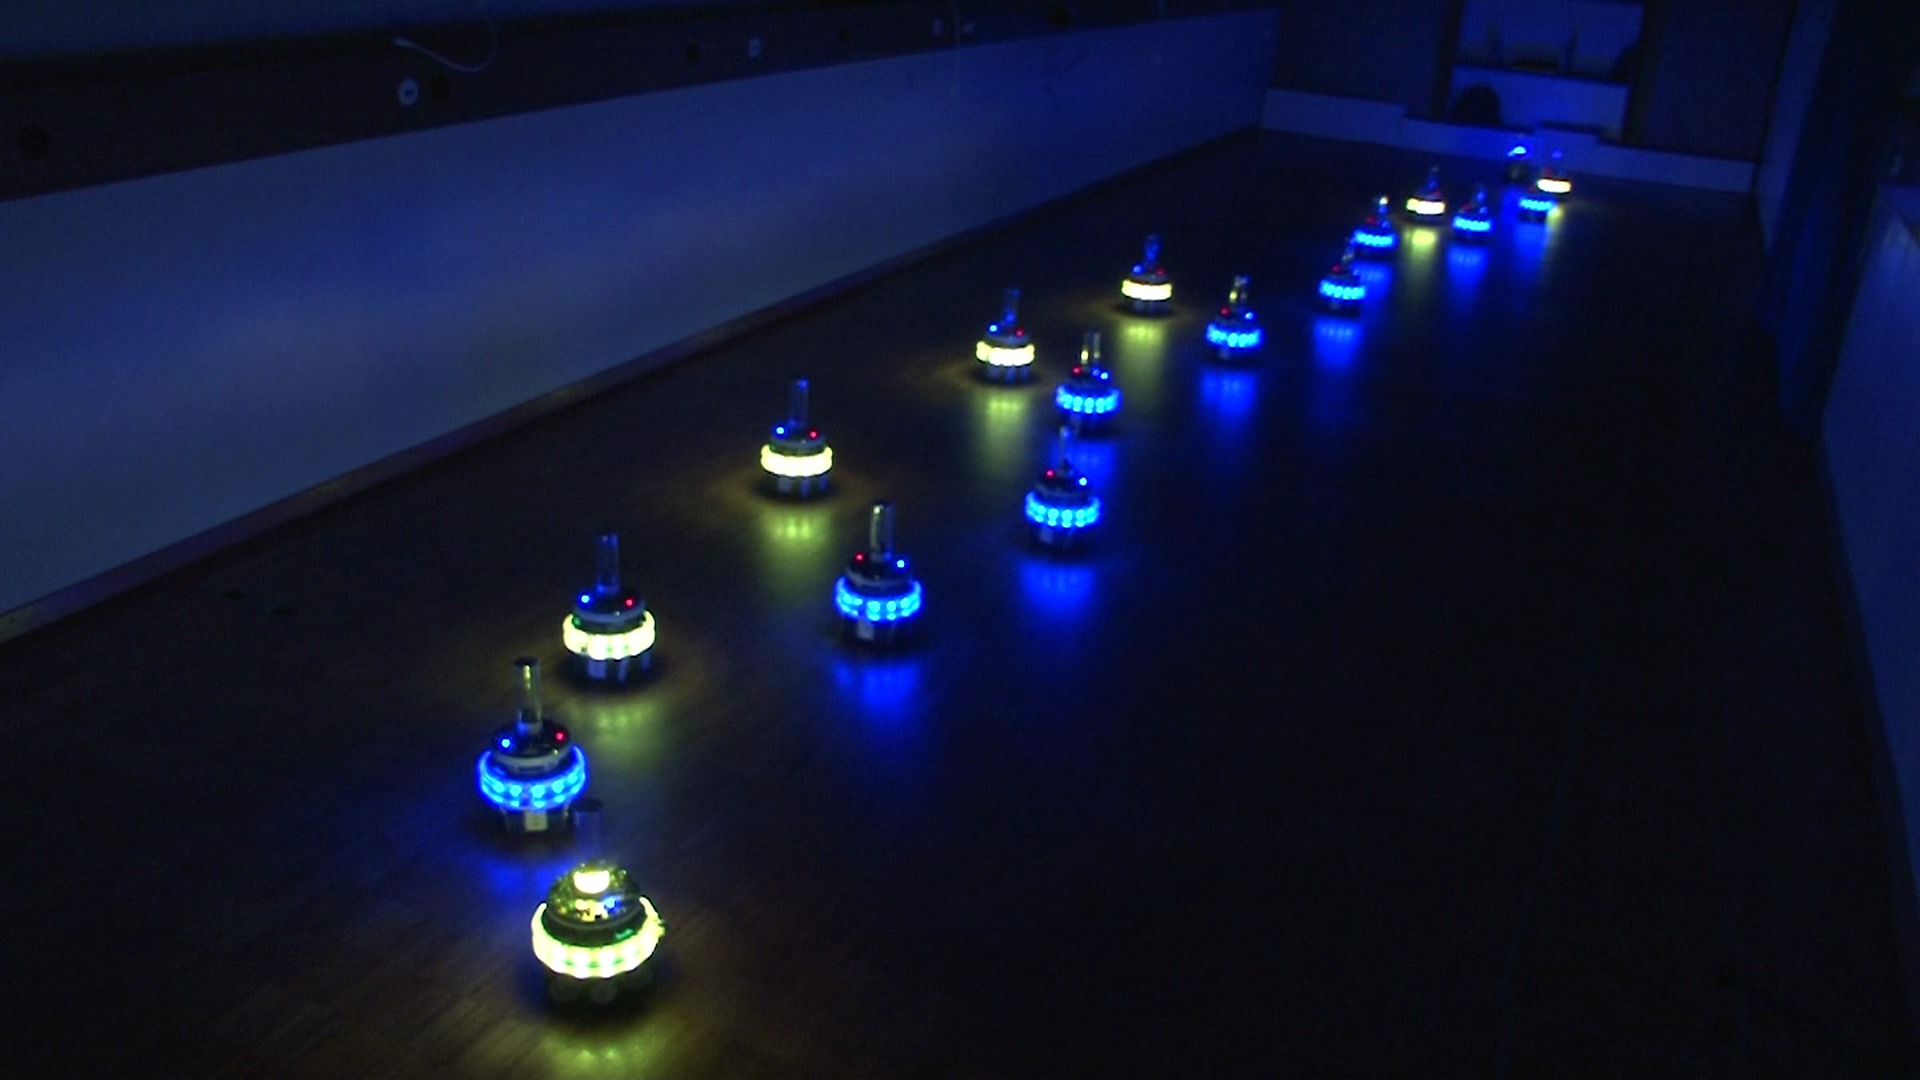
\includegraphics[height=1.6cm]{img/navigation.jpg}
	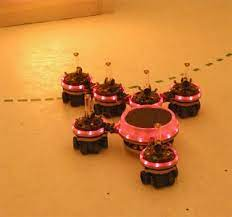
\includegraphics[height=1.6cm]{img/transportation.jpeg}
	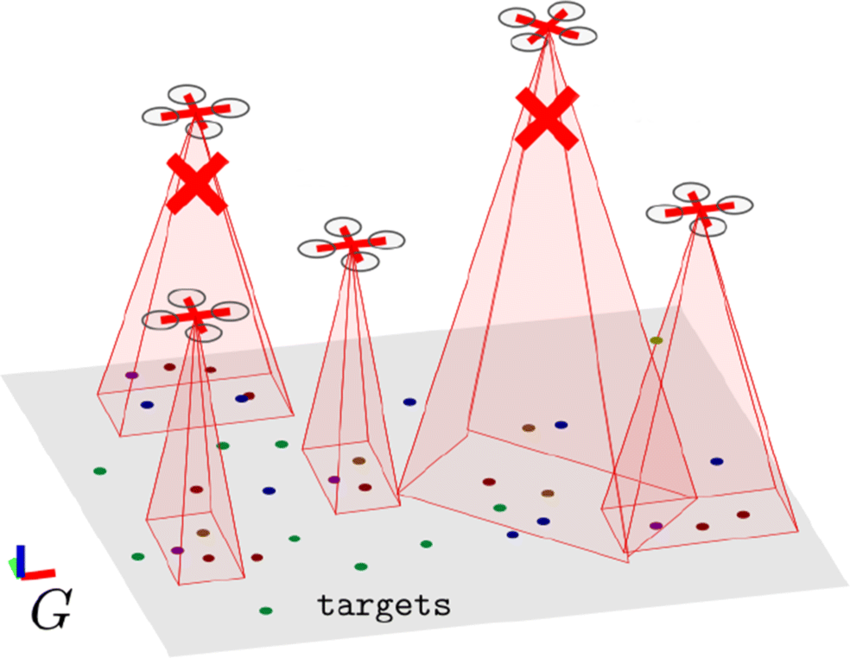
\includegraphics[height=1.6cm]{img/localization.png}
	\end{center}
	\end{frame}
	\begin{frame}{Programming Swarms}
		\begin{exampleblock}{Solutions}
			\begin{itemize}
					\item Bottom-up approach: mimicking nature by programming individual agents.
					\begin{itemize}
						\item \textbf{Swarm Intelligence} (SI): a computational paradigm inspired by the collective behaviour of social insects.
					\end{itemize}
					\item Top-down -- macroprogramming: collective abstractions as first-class citizens of the programming model.
					\begin{itemize}
						\item \alert{Centralized -- orchestration}: a single entity coordinates the swarm through a task description
						\item \alert{Decentralized}: agents interact locally to achieve a global goal
						\begin{itemize}
							\item \emph{Buzz}: a practical macroprogramming model for swarm robotics.
							\item \textbf{Aggregate programming}: a programming language for self-organizing systems.
						\end{itemize}
					\end{itemize}
			\end{itemize}
		\end{exampleblock}
	\end{frame}
%%%%%%%%%%%%%%%%%%%%%%%%%%%%%%%%%%%%%%%%%%%%%%%
%%%%%%%%%%%%%%%%%%%%%%%%%%%%%%%%%%%%%%%%%%%%%%%
%%%%%%%%%%%%%%%%%%%%%%%%%%%%%%%%%%%%%%%%%%%%%%%
\begin{frame}[fragile]{Aggregate computing -- one slide}
	
	\metroset{block=fill}
	\hsplit{

  \begin{exampleblock}{\footnotesize Self-org-like computational model}
		\scriptsize
		\alert{interaction:} \emph{repeated} msg exchange with \bo{neighbors}
		\\[-0.05cm]%
		\alert{behavior:} \emph{repeated} execution of \underline{async rounds}%
		\\[-0.05cm]%
		%\alert{formal model of executions:} event structures 
	\end{exampleblock}
	\begin{exampleblock}{\footnotesize Programming Model}
	\scriptsize

	\alert{formal core language:} field calculus
	\\[-0.05cm]
	\alert{paradigm:} \bo{functional, macro-programming}

	\centering
	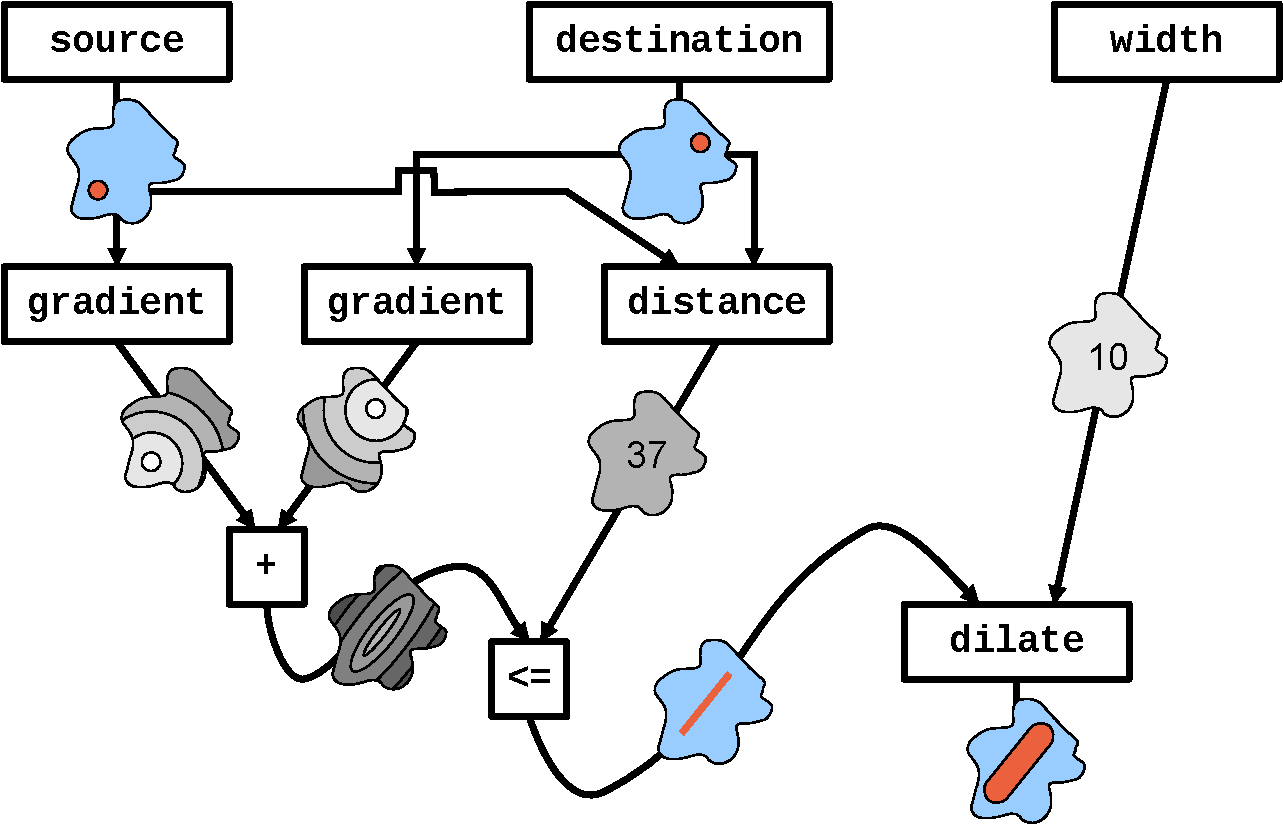
\includegraphics[height=0.33\textheight]{img/channel.pdf}
	\end{exampleblock}	
		}{
		\begin{exampleblock}{\footnotesize Why?}
			\scriptsize
		
			\alert{\faThumbsUp} \, Scale naturally with nodes in the systems\\[-0.05cm]
			\alert{\faThumbsUp} \, High-level abstractions to devise applications
			\\[-0.05cm]
			\alert{\faThumbsUp} \, Decentralized, self-organizing systems
			\\[-0.05cm]
			\alert{\faThumbsUp} \, Existing framework support swarm programmings
			%\lbl{semantics:} (1) device; (2) network; (3) global comp.
		\end{exampleblock}
		
  
		\begin{exampleblock}{\footnotesize Collective Abstractions} %{Engineering approach}
			\scriptsize
		\alert{abstraction:} \bo{computational fields} ($\mathit{dev/evt} \mapsto \mathbb{V}$) \vspace{0.1cm}
			\alert{examples:} \bo{temperature fields}, \bo{actuation fields} \vspace{0.1cm}
			\begin{center}
				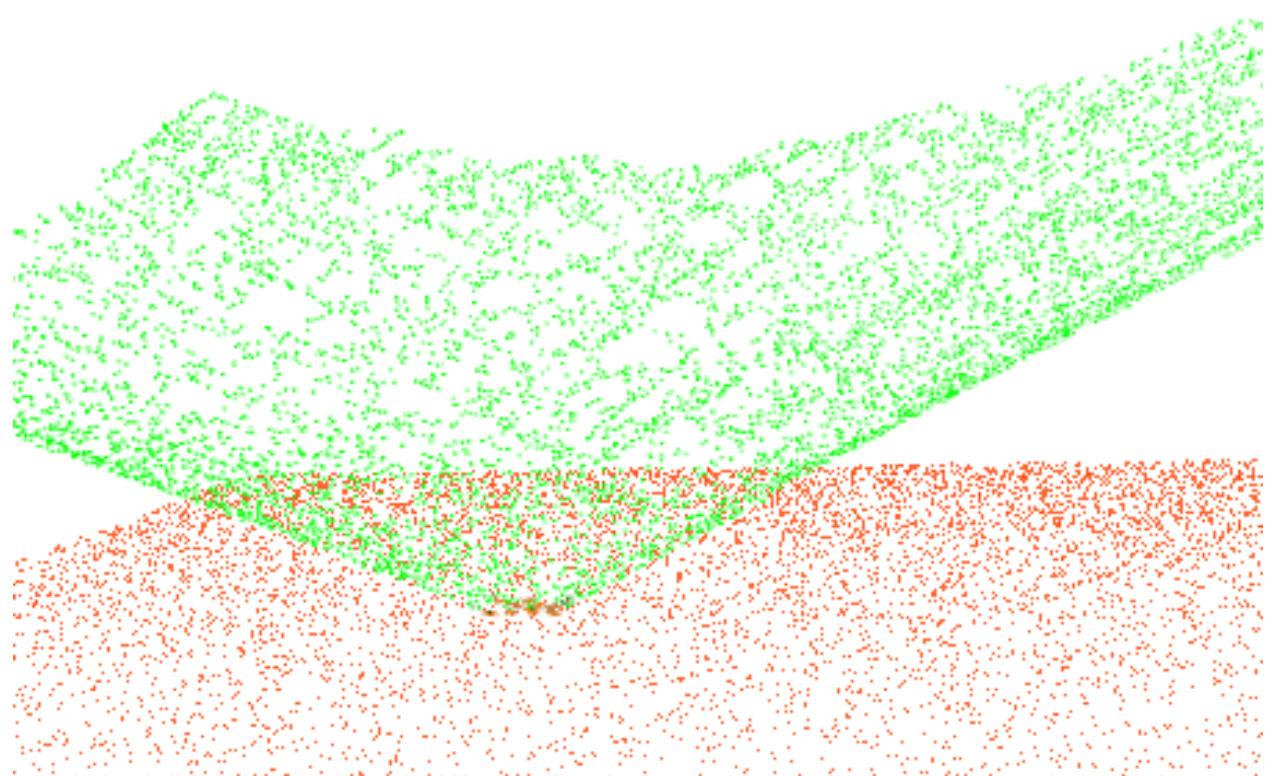
\includegraphics[width=0.3\textwidth]{img/3d-gradient.png}
				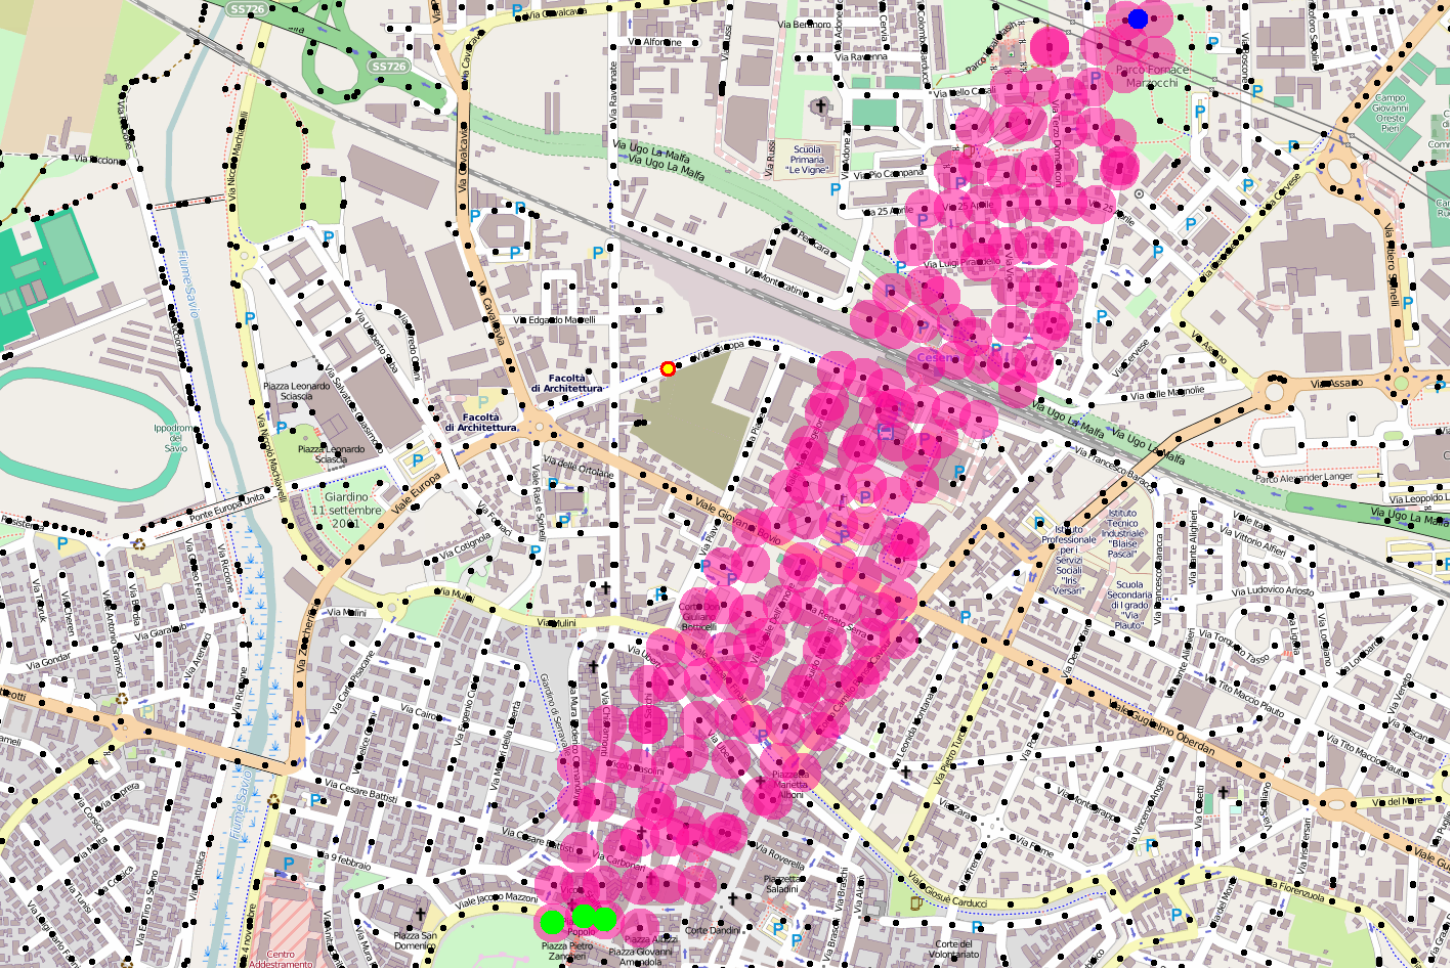
\includegraphics[width=0.28\textwidth]{img/channel.png}
				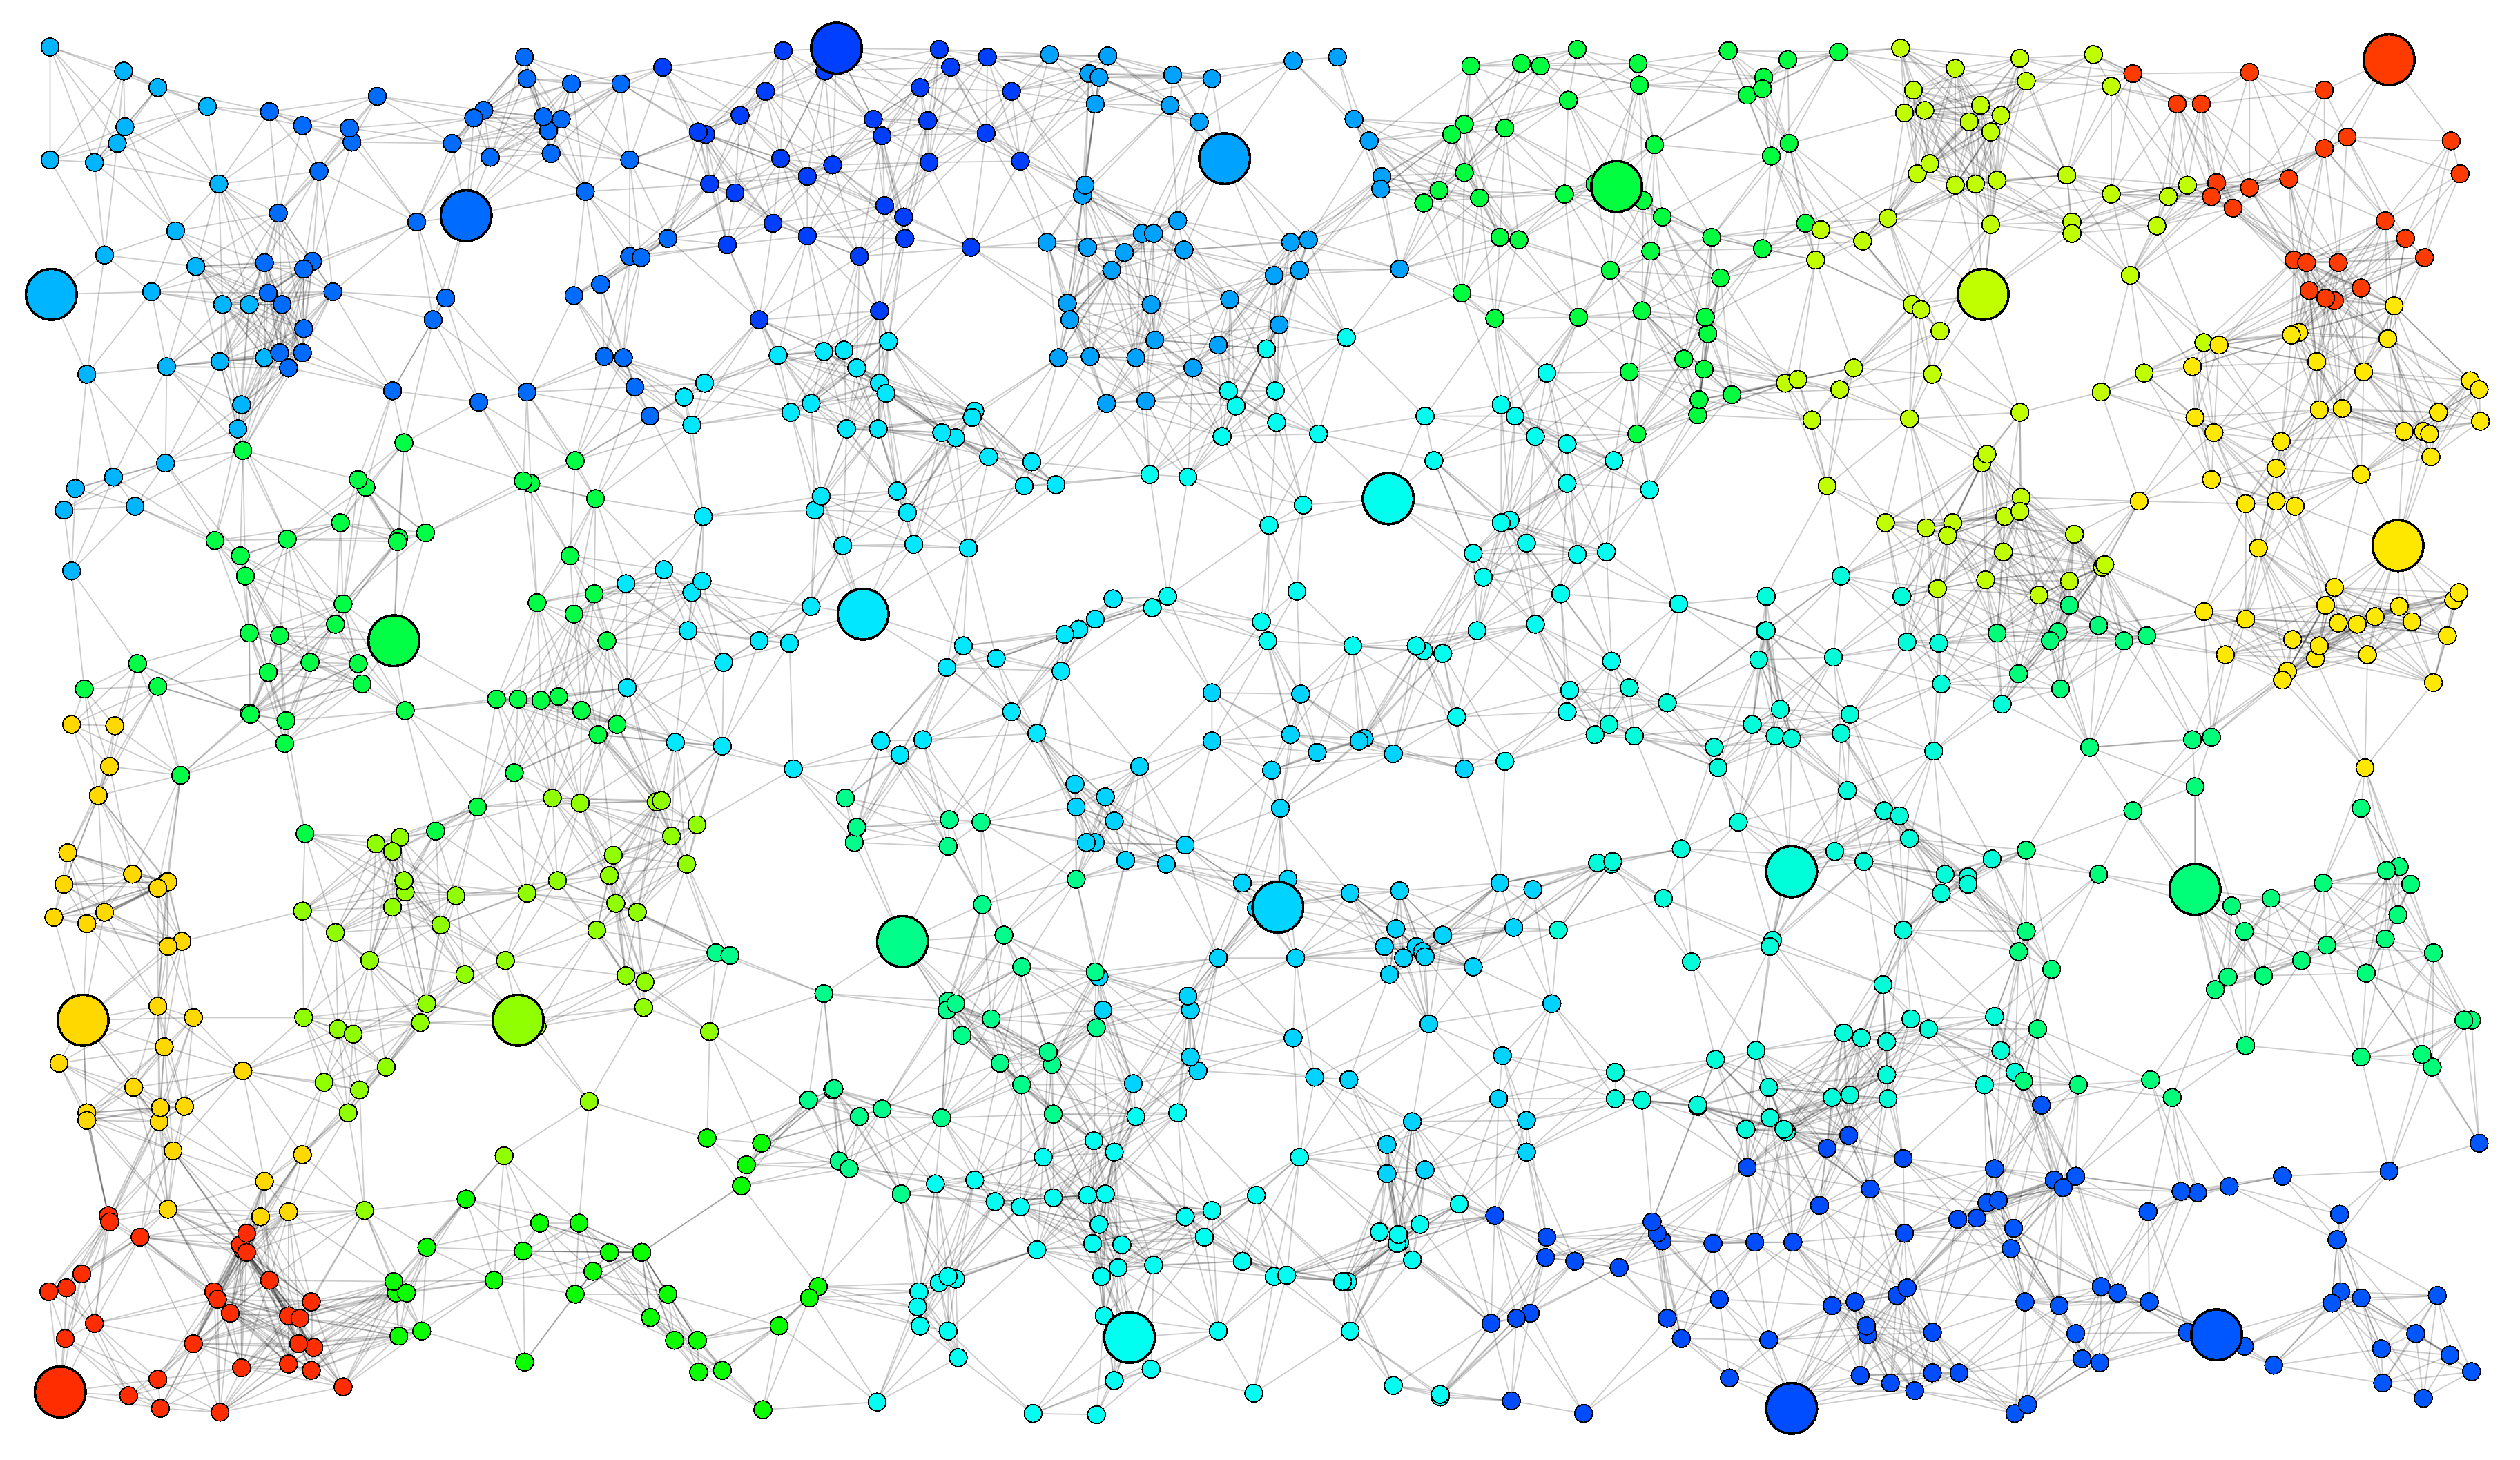
\includegraphics[width=0.3\textwidth]{img/scr-result.png}
				\end{center}
		%\tiny \fullcite{bpv:aggregate:programming}
		\end{exampleblock}
		%}
 }
	
\end{frame}
\begin{frame}{Accessibility to Aggregate Computing}
	\begin{block}{Problem}
		\begin{itemize}
			\item \alert{Steep learning curve} for non-experts
			\item \alert{High cognitive load} in designing and debugging
			\item \alert{Lack of visual support} for understanding and debugging
		\end{itemize}
	\end{block}
	How to make aggregate computing accessible to non-experts?
\end{frame}
\begin{frame}{Requirements}
	\begin{enumerate}
    \item \textbf{User-Friendly Interface:} Drag-and-drop for accessibility.
    \item \textbf{Rapid Feedback Loop:} Instant execution for faster learning.
    \item \textbf{Knowledge Transfer:} Visual to textual code for deeper understanding.
    \item \textbf{Compositional Approach:} Building complexity from simple blocks.
    \item \textbf{Minimalist Design:} Curated blocks for focused design.
    \item \textbf{Engagement and Fun:} Interactive environment for enjoyable learning.
\end{enumerate}

\end{frame}
\begin{frame}[standout]
	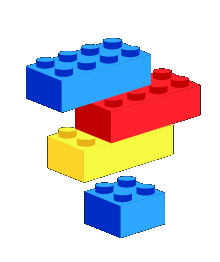
\includegraphics[width=1cm]{img/scafiblocks-logo.png}
	\Huge{\textbf{ScaFi-Blocks}}
	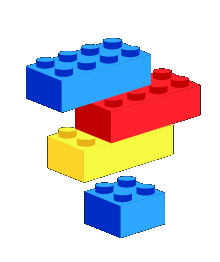
\includegraphics[width=1cm]{img/scafiblocks-logo.png}
	\Large{
		\begin{itemize}
			\item \alert{Visual programming environment} for aggregate computing based on ScaFi
			\item \alert{Low-code} approach to swarm design
			\item \alert{Interactive} and \alert{intuitive} design and debugging
		\end{itemize}}
\end{frame}
\begin{frame}{ScaFi Blocks -- Components}
	\begin{itemize}
		\item \alert{Block Library:} Curated set of blocks for aggregate computing.
		%\begin{itemize}
		%	\item Conditions: if-else blocks
		%	\item Actuations: change the environment (movement and leds)
		%	\item Sensing: perceive the environment (boolean sensors)
		%	\item Aggregate computing primitives: gradient, broadcast, collect, etc.
		%	\item API Examples: swarming behaviors 
		%\end{itemize}

		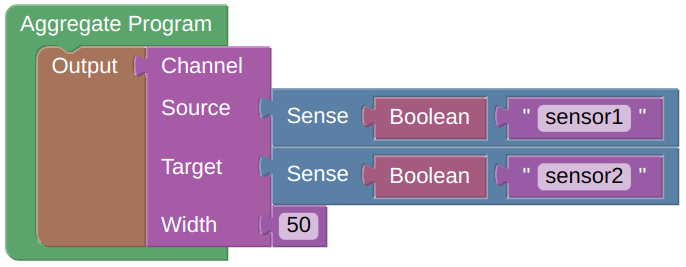
\includegraphics[width=0.5\textwidth]{img/channel-visual.png}
		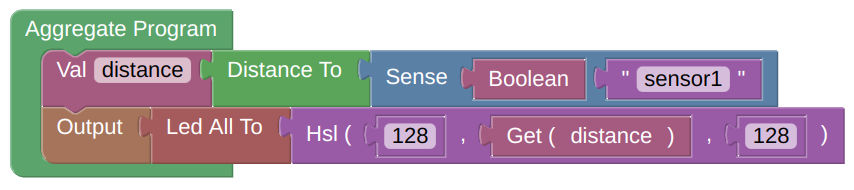
\includegraphics[width=0.5\textwidth]{img/distance-example.png}
		
		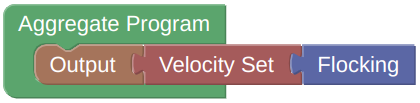
\includegraphics[width=0.25\textwidth]{img/movement-example.png}
		\item \alert{Workspace:} Drag-and-drop interface for designing swarm behaviors (based on Blockly)
		\item \alert{Simulator:} Instant execution of the designed behavior (based on ScaFi Web)
	\end{itemize}
\end{frame}
\begin{frame}{ScaFi-Blocks -- Architecture}
	\centering
	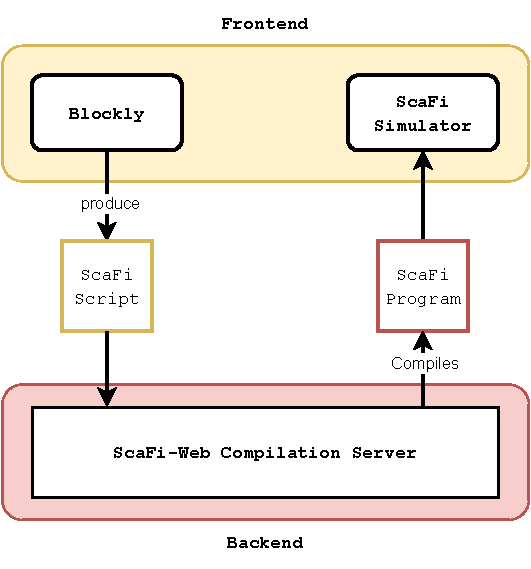
\includegraphics[width=0.5\textwidth]{img/scafi-blocks-architecture.drawio.pdf}
\end{frame}

\begin{frame}{ScaFi-Blocks -- Interface}
	\centering
	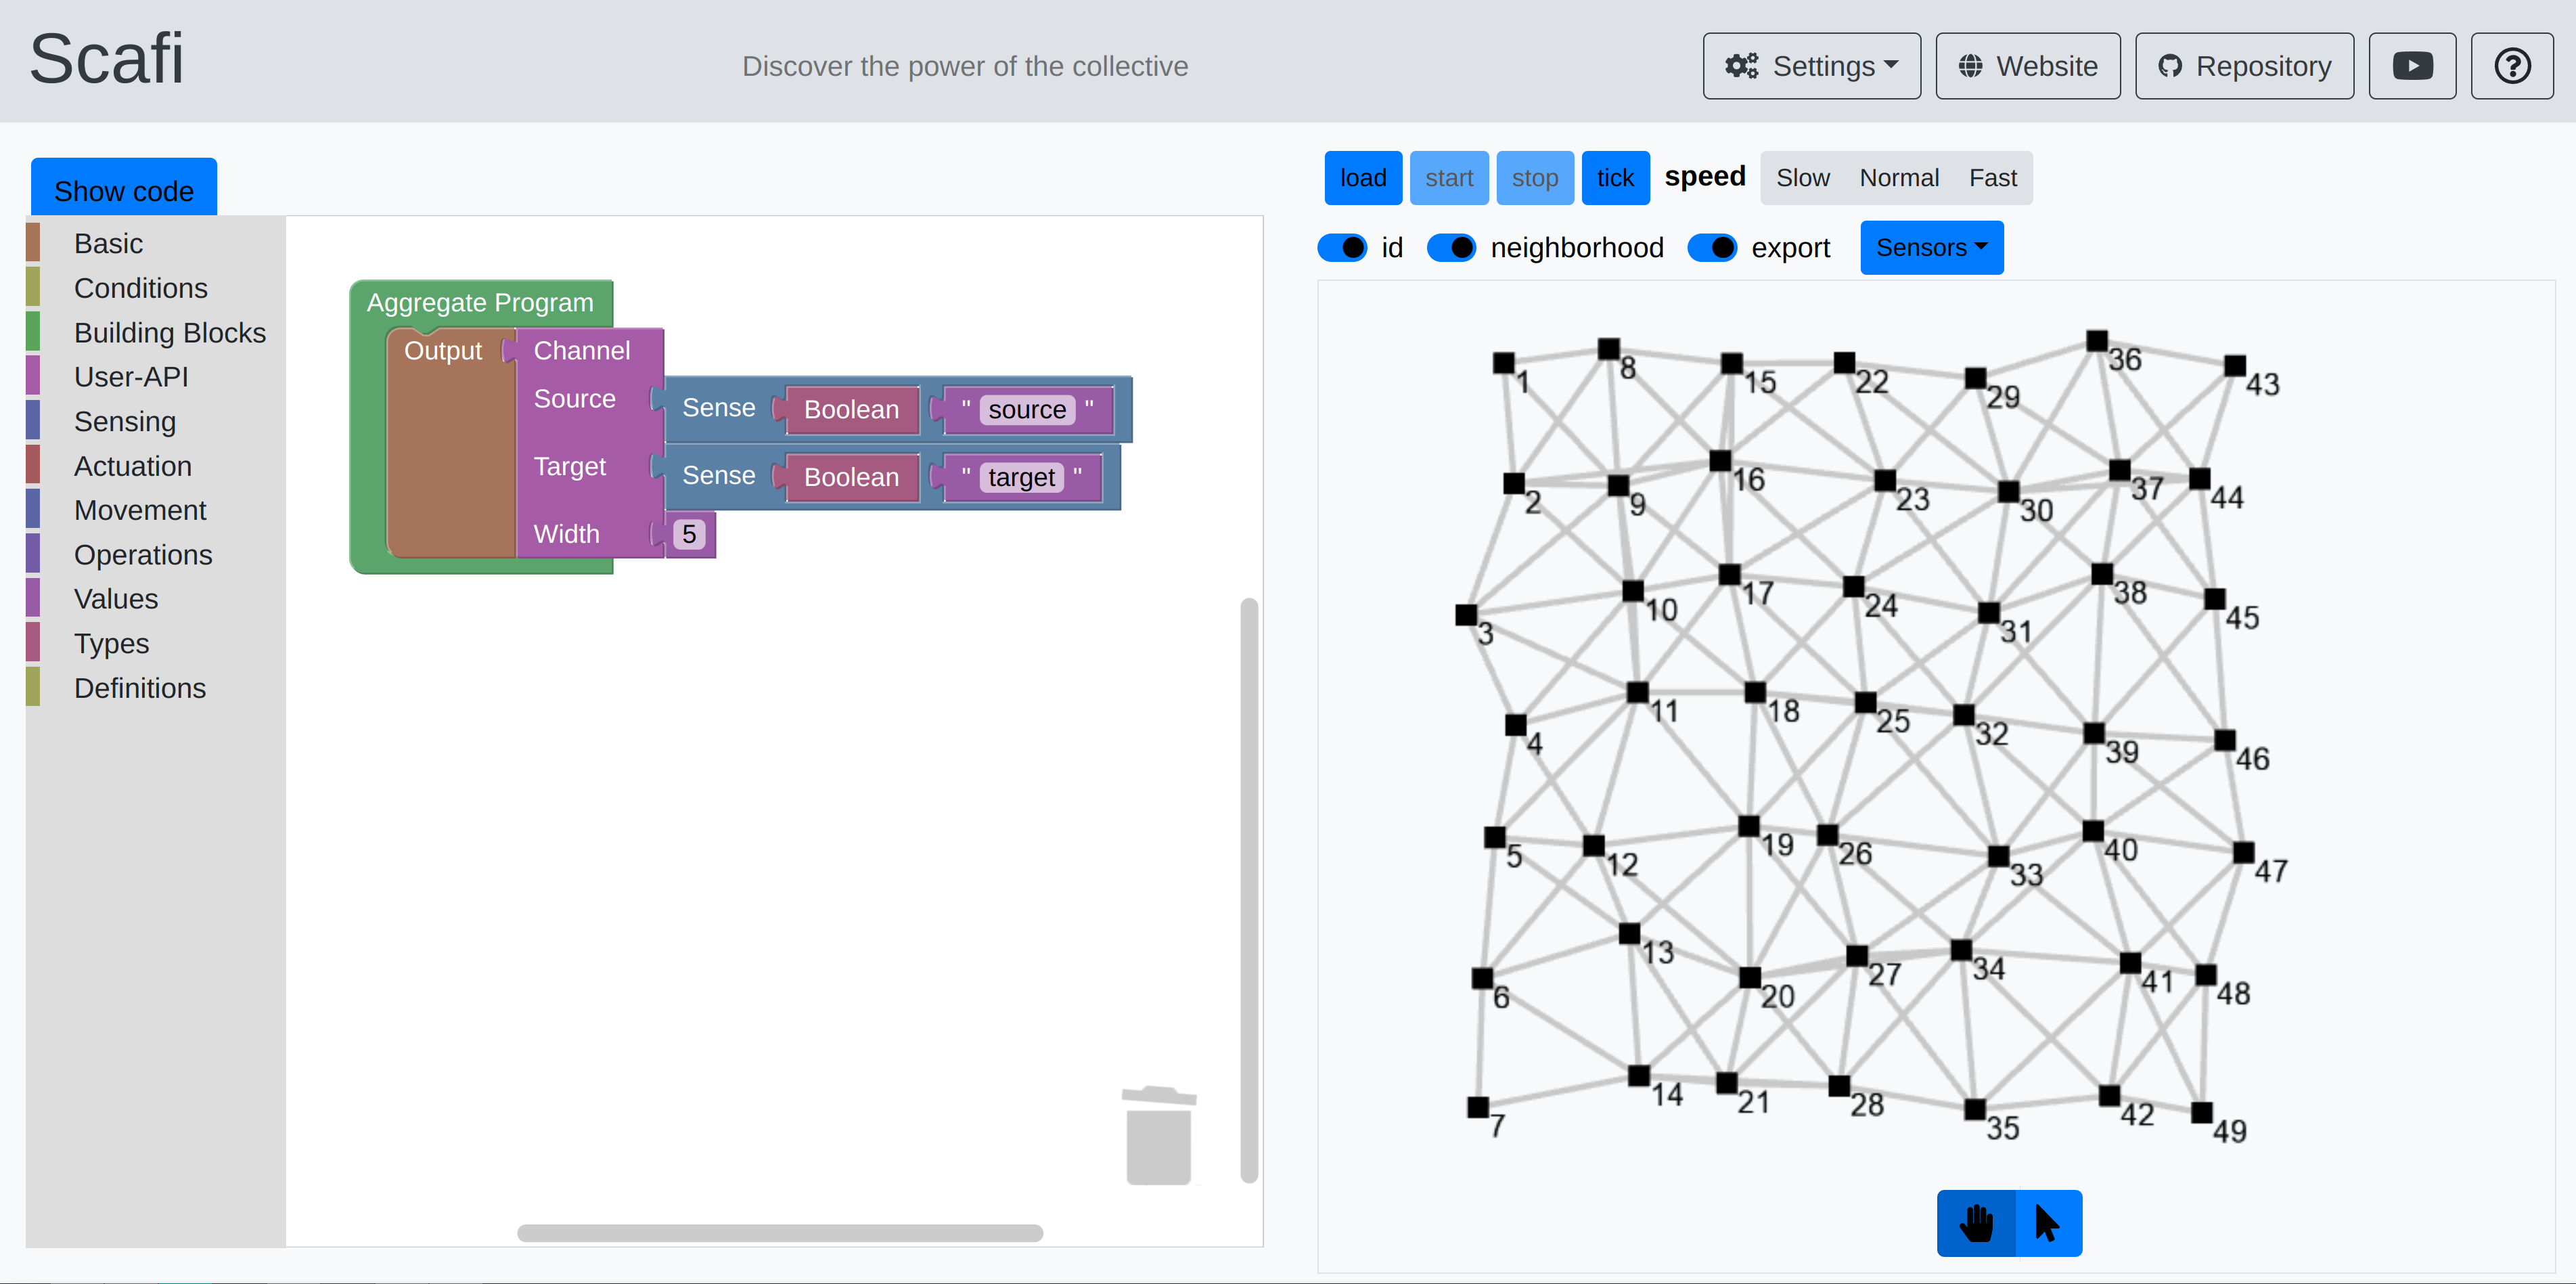
\includegraphics[width=\textwidth]{img/scafiblocks.png}
\end{frame}
\begin{frame}[standout]
	\Huge\textbf{Demo}
\end{frame}
\begin{frame}{Conclusion}
\begin{itemize}
	\item \alert{Swarm programming} is a promising paradigm for self-organizing systems.
	\item \alert{Aggregate computing} provides a formal model for swarm programming.
	\item \alert{ScaFi-Blocks} is a visual aggregate programming environment for low-code swarm design.
	\begin{itemize}
		\item \alert{User-friendly interface} for non-experts
		\item \alert{Rapid feedback loop} for faster learning
		\item \alert{Knowledge transfer} from visual to textual code
	\end{itemize}
	\begin{exampleblock}{Future Works}
		\begin{itemize}
		\item \textbf{Evaluation} with non-experts
		\item \textbf{Integration} with real robots
		\item \textbf{Extension} to more complex behaviors
		\end{itemize}
	\end{exampleblock}
\end{itemize}
\end{frame}
\end{document}

